\chapter{디지털 비디오 인터페이스}
\begin{figure*}
    \centering
    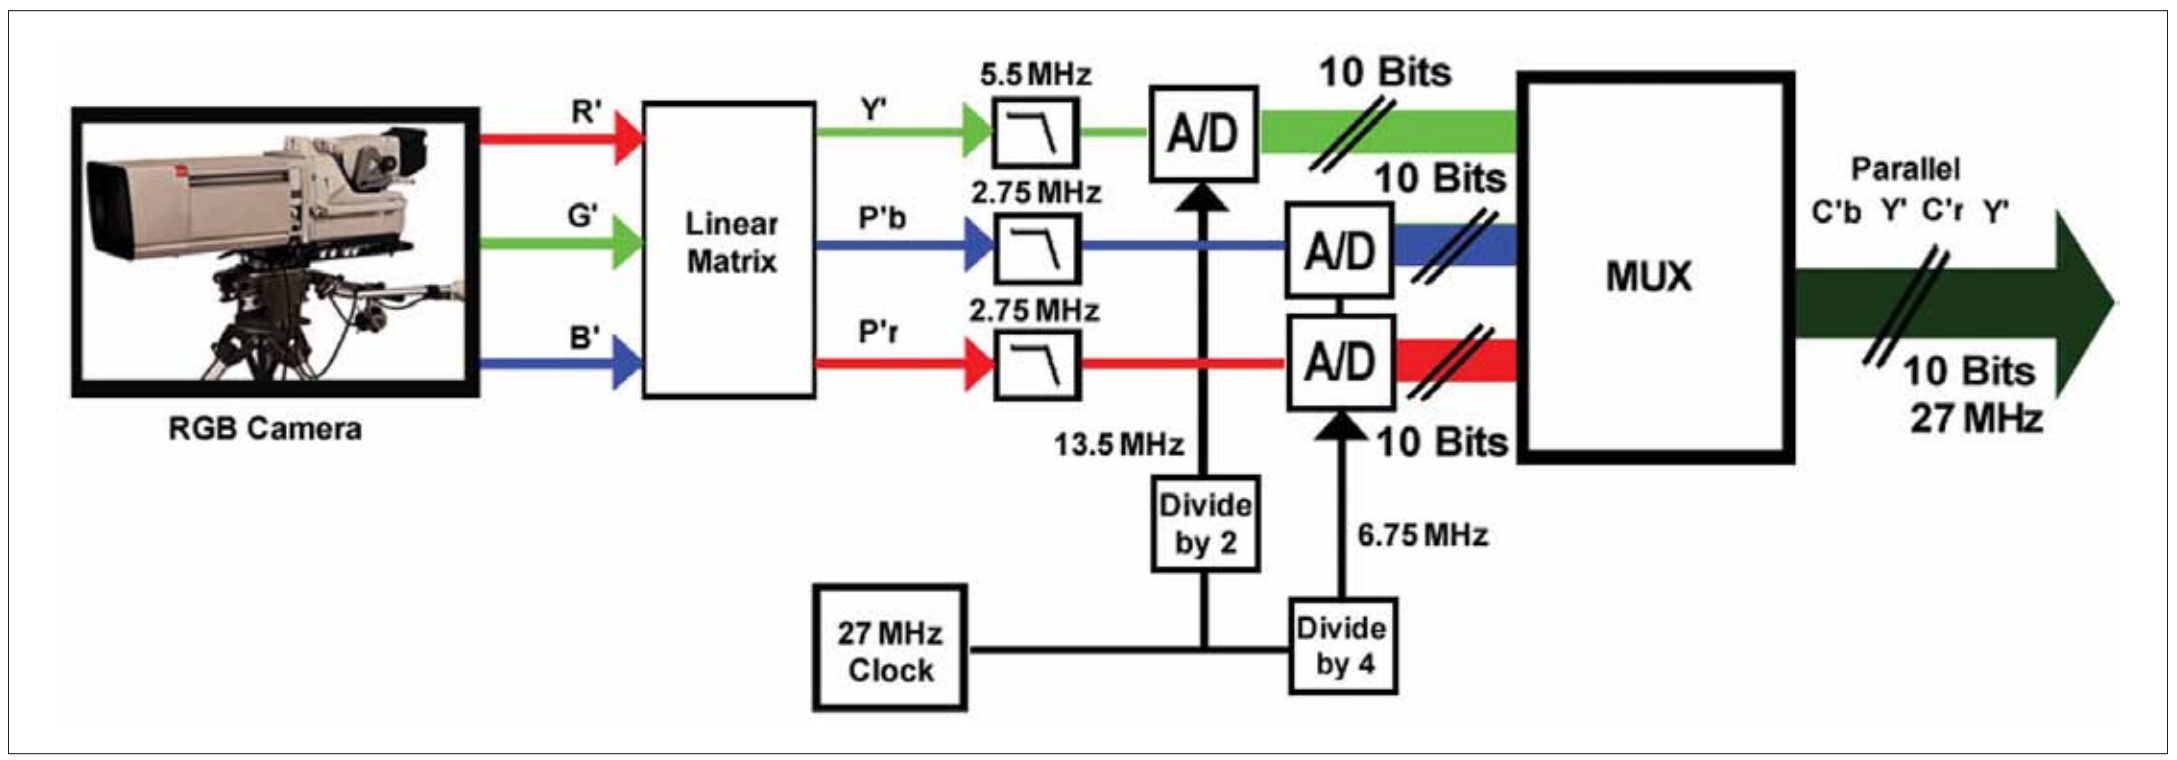
\includegraphics[width=\textwidth]{digitizing rgb camera.PNG}
    \caption{RGB 카메라 신호의 디지털화}\label{fig:digitizing rgb camera}
\end{figure*}
이 시점에서 아날로그 비디오와 연결하는 디지털 인터페이스를 간단히 살펴보는 게 적절하다.
\figurename~\ref{fig:digitizing rgb camera}부터 \figurename~\ref{fig:recovering analog values from prallel data}까지의 블록 다이어그램은 비디오 프로덕션 장비가 디지털 비디오 요소들을 어떻게 다루는지 이해하는 데 도움을 줄 것이다.
이 그림들이 SD 시스템을 다루긴 하지만, 기본 개념은 HD 포맷에서도 똑같다. HD 포맷에서는 샘플링과 데이터 속도가 더 빠르고 각각 분리된 10비트의 휘도와 색차 버스가 시스템 전체에서 더 유지되고, 이를 통해서 고속으로 작동해야 하는 회로를 줄인다.
\\
감마 보정된 RGB(\figurename~\ref{fig:digitizing rgb camera})는 선형 행렬을 통해서 휘도 요소인 Y'과 두 개의 배율이 곱해진 색차 요소인 P'b와 P'r로 바뀐다.
눈은 색상 변화보다 밝기 세부 정보의 변화에 더 민감하므로, Y'신호는 시스템 내에서 더 높은 대역폭으로 전달된다(SD의 경우 5.5 MHz).
휘도와 색차 신호는 샘플링(디지털화) 과정에서 에일리어싱을 일으킬 수 있는 고주파 비디오 성분을 제거하기 위해서 저역 통과 필터로 처리된다.
필터링된 휘도 신호는 아날로그-디지털 변환기에서 13.5 MHz의 속도로 샘플링되어 13.5 Mb/s의 10비트 데이터 스트림으로 바뀐다.
두 개의 색차 신채널들은 필터링된 후 아날로그-디지털 변환기에서 6.75 MHz의의 속도로 2개의 6.75 Mb/s의 데이터 스트림으로 바뀐다.
세 비디오 채널들은 27 Jb/s의 단일 10비트 병렬 데이터 스트림으로 다중화되어 합쳐진다.
\\
\begin{figure*}
    \centering
    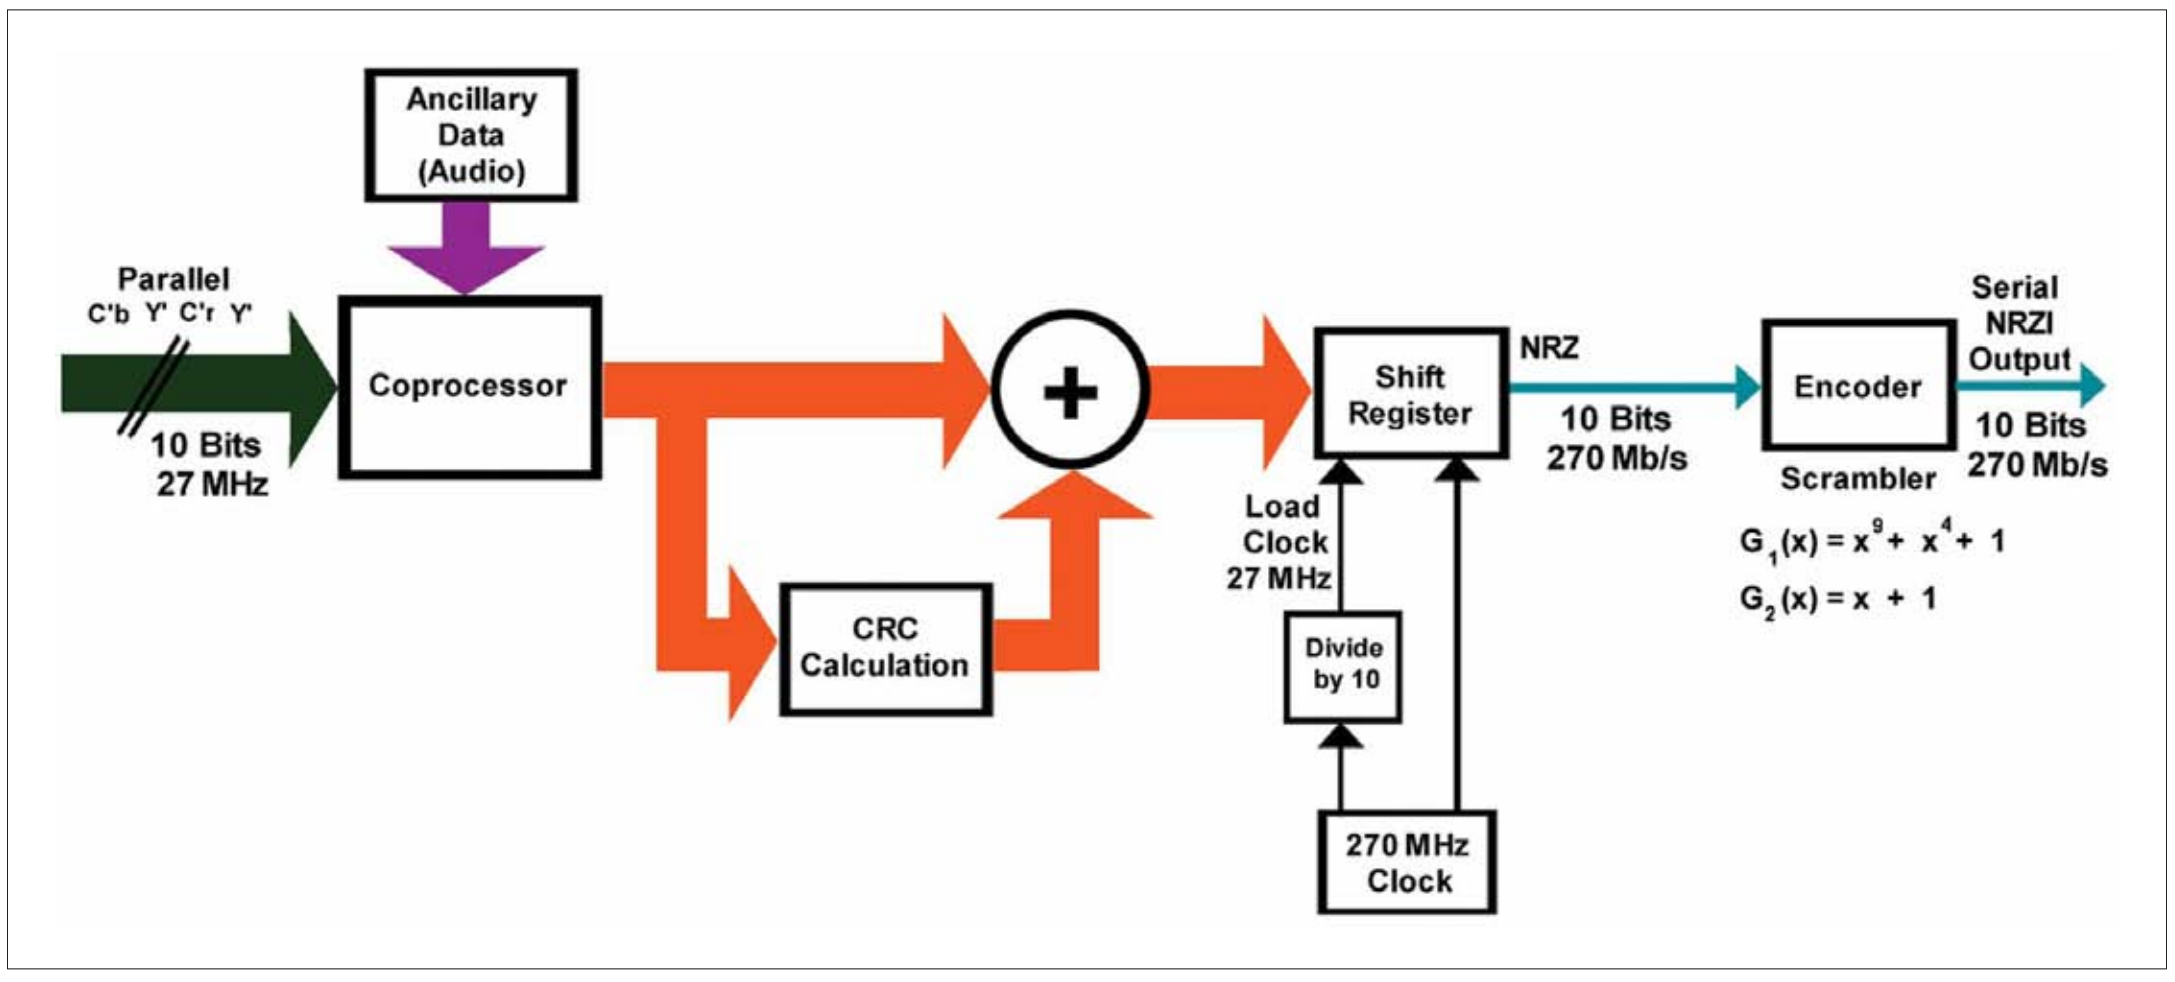
\includegraphics[width=\textwidth]{processing and serializing parallel data stream.PNG}
    \caption{병렬 데이터 스트림의 처리와 직렬화}\label{fig:processing and serializing parallel data stream}
\end{figure*}
보조 처리기(\figurename~\ref{fig:processing and serializing parallel data stream})가 타이밍 기준 신호, AES/EBU 포맷의 디지털 오디오와 기타 부가 데이터를 추가한다. 데이터에 대한 체크섬 또한 계산되어서 병렬 데이터 스트림에 추가된다.
\\
27 Mb/s, 10 비트의 병렬 데이터는 270 Mb/s로 작동하는 시프트 레지스터(또는 직렬화기)로 입력되어서, 이 예제에서는 SD 표준인 ITU-R BT-656/SMPTE 259M을 따르는 적절한 전송을 위해서 스크램블된다.
\\
SD ITU-R BT-656/SMPTE 259M 적합 신호는 표준 비디오 케이블을 따라서 거의 100\%의 무결성을 유지하며 300 m를 갈 수 있다. 1.485 Gb/s의 HD SMPTE 292M 적합 신호는 약 100 m를 갈 수 있다.
\\
\begin{figure*}[!t]
    \centering
    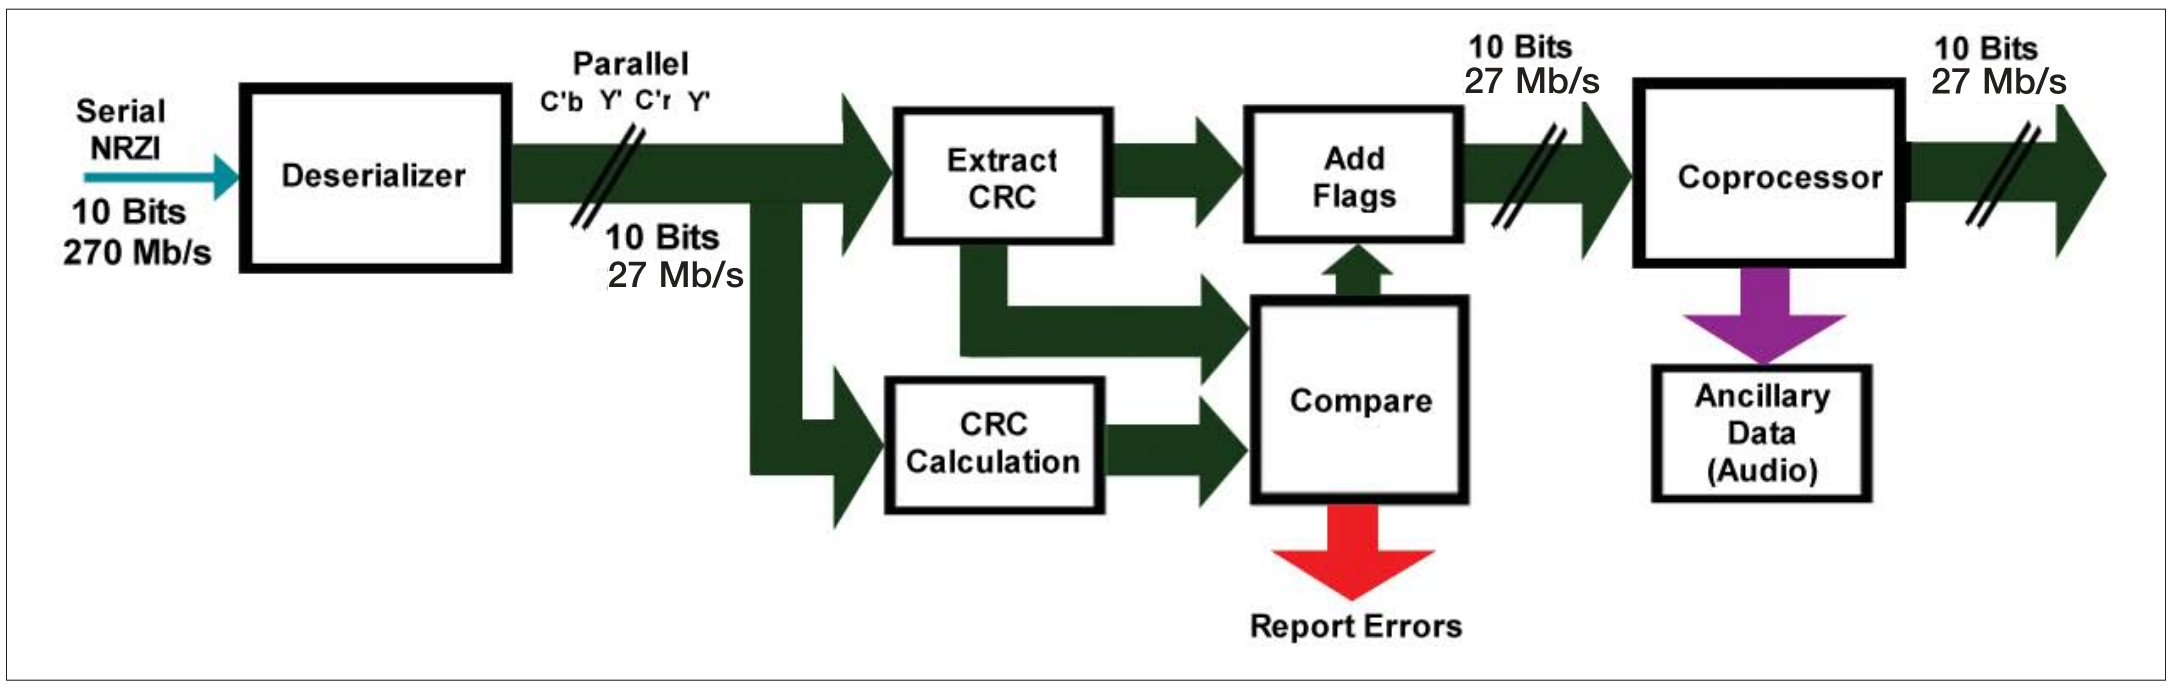
\includegraphics[width=\textwidth]{sdi receiver.PNG}
    \caption{SDI 수신기 - 비디오 데이터를 역직렬화하여 다시 병렬로 만든다}\label{fig:sdi receiver}
\end{figure*}
\begin{figure*}[h!]
    \centering
    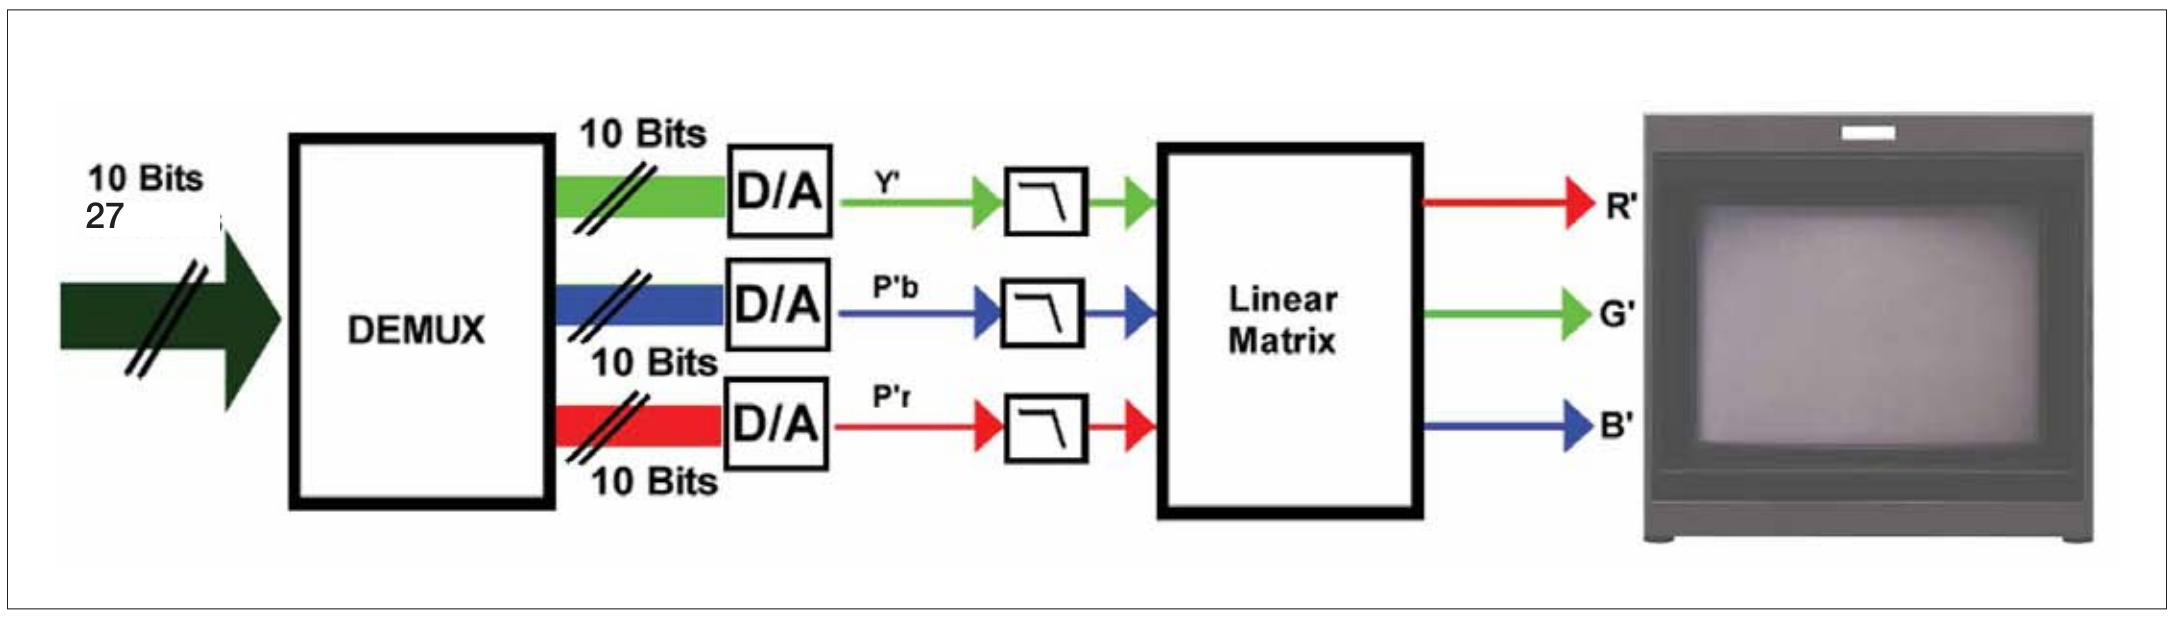
\includegraphics[width=\textwidth]{recovering r'g'b' from parallel data.PNG}
    \caption{병렬 데이터에서 아날로그 R'G'B'를 복원}\label{fig:recovering analog values from prallel data}
\end{figure*}
수상기에서는(\figurename~\ref{fig:sdi receiver}) 절반 클럭 주파수의 에너지가 감지되어서 270 Mb/s로 입력되는 신호를 적절히 아날로그 등화 처리한다. 새로운 270 MHz 클럭이 NRZI(Non-Return to Zero Inverse) 신호의 에지에서 복원되고, 등화된 신호가 논리 상태를 결정하기 위해서 샘플된다.
역직렬화기는 인코더의 스크램블 알고리즘의 역변환을 이용해서 스크램블을 해제하여 27 Mb/s의 10비트 데이터 스트림을 만든다. 임베디드된 체크섬이 수신기에서 추출되어서 수신된 데이터로부터 새로 계산된 체크섬과 비교되어 오류가 발생했는지 확인하고 적절한 플래그를 데이터 스트림에 붙인다.
보조 처리기는 오디오나 다른 부가 데이터들을 추출한다.
\\
10비트 데이터 스트림은 역다중화되어(\figurename~\ref{fig:recovering analog values from prallel data}) 디지털 휘도와 색차 스트림이 되고, 3개의 디지털-아날로그 변환기를 통하여 아날로그 신호가 되며, 이산적인 데이터 레벨에서 부드러운 아날로그 신호가 되도록 (역자 주:저역) 필터를 통과하고 디스플레이에서 원래의 R'G'B'신호가 되게 행렬을 이용해서 합쳐진다.
\\
이 간단한 시스템 개관은 시스템이 어떻게 작동하는지 이해하는 데 도움이 될 것이다. 추가적인 디지털 인터페이스에 대한 세부적인 설명은 뒤의 문단들에서 나올 것이다.

\section{601 샘플링}
\begin{figure*}[t!]
    \centering
    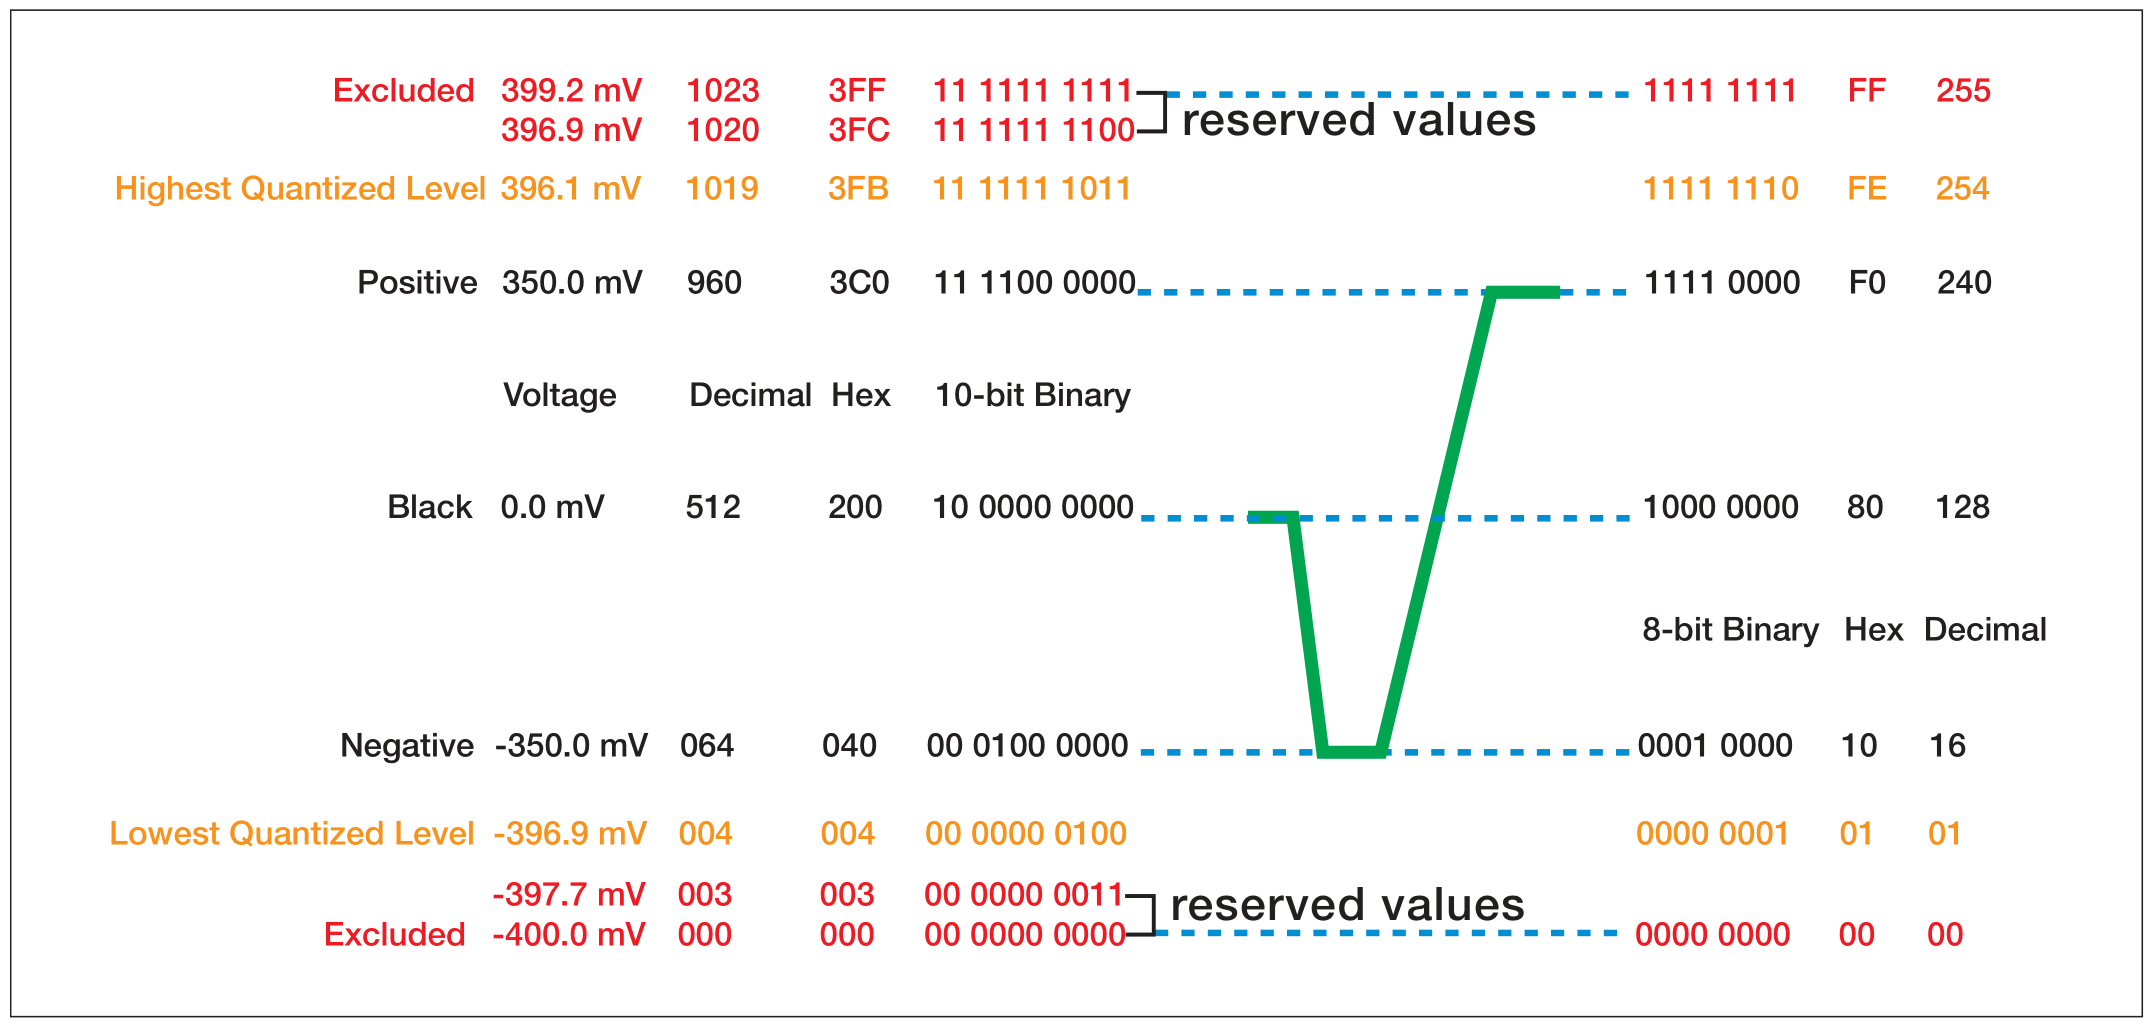
\includegraphics[width=\textwidth]{color difference quantizing.PNG}
    \caption{색차 신호의 양자화}\label{fig:color difference quantizing}
\end{figure*}
\begin{figure*}[h!]
    \centering
    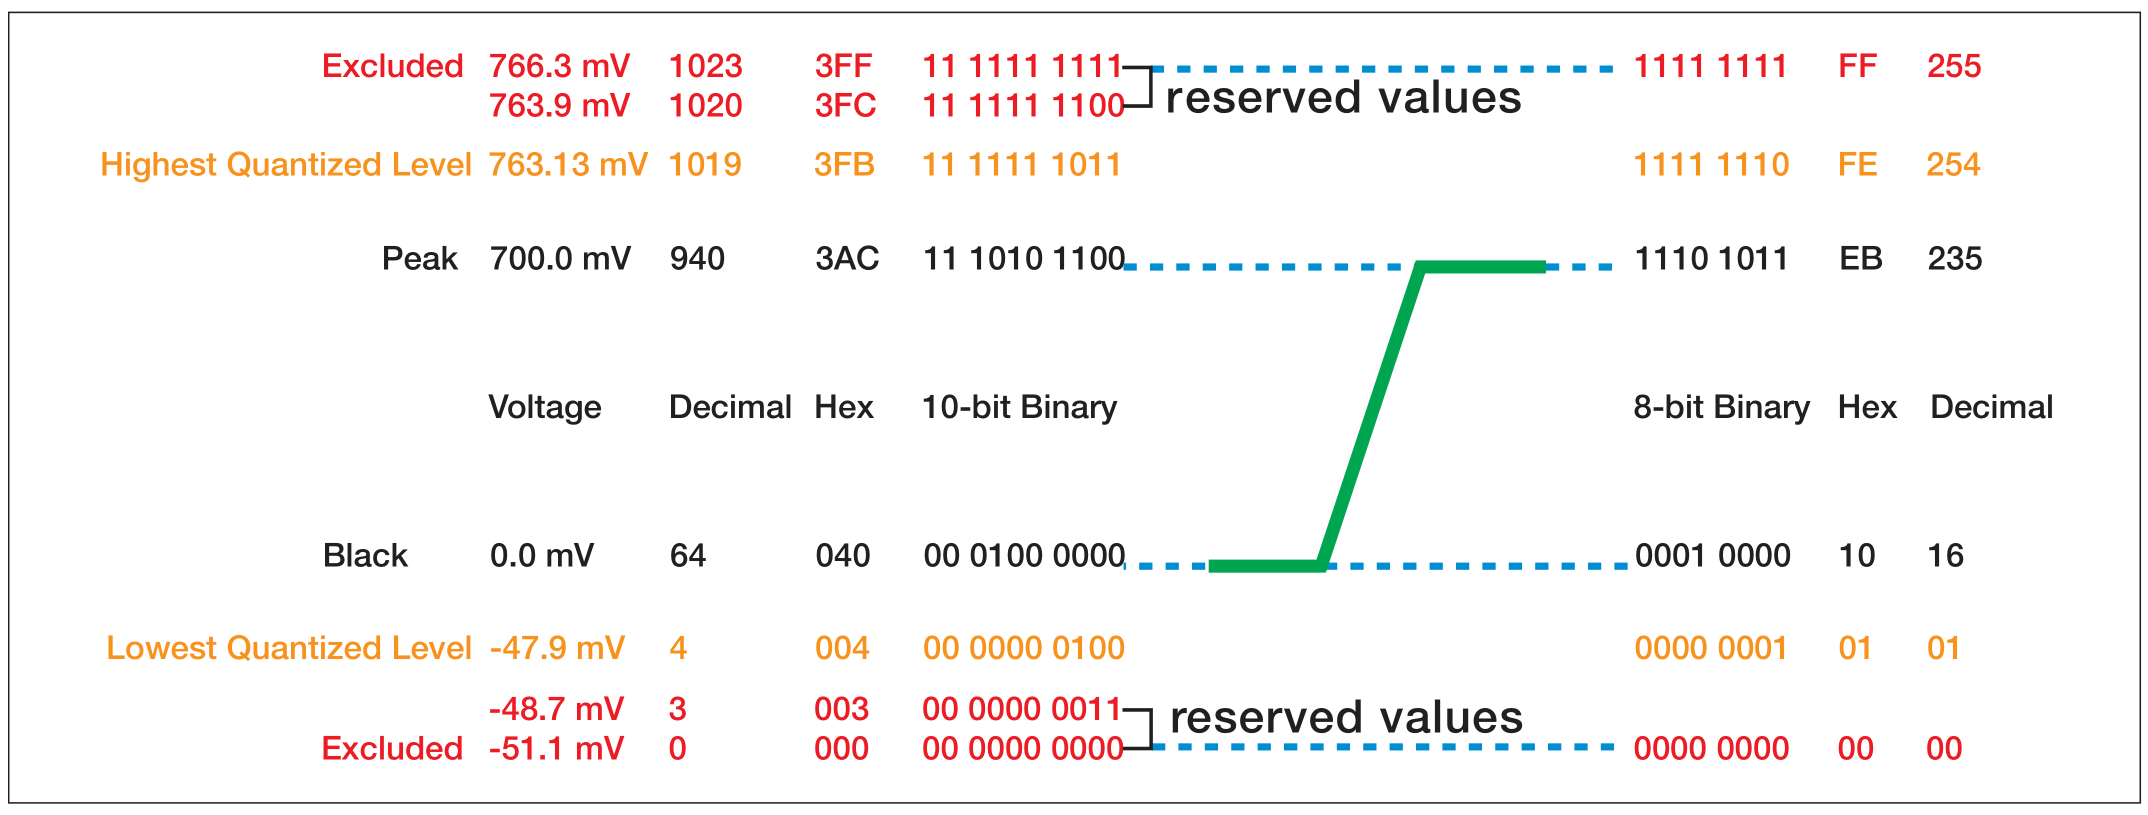
\includegraphics[width=\textwidth]{luminance quantizing.PNG}
    \caption{휘도 신호의 양자화}\label{fig:luminance quantizing}
\end{figure*}
ITU-R BT.601은 625/50과 525/60 텔레비전 시스템의 디지털 요소들에 대한 파라미터를 결정하기 위한 연합 SMPTE/EBU 태스크 포스에서 만들어진 샘플링 표준이다.
이 작업은 1981년에 SMPTE에 의해 후원된 일련의 테스트들로 완결되었고, 잘 알려진 CCIR 권고안 601 (이제는 ITU-R BT.601)이라는 결과가 나왔다.
이 표준 문서는 525와 625줄 신호에서 사용되는 샘플링 방법을 규정한다. 이는 아날로그 휘도에 대한 13.5 MHz와 두 개의 아날로그 색상차 신호에 대한 6.75 MHz의 직교 샘플링을 규정하고 있다.
샘플링된 값들은 디지털 휘도인 Y'와 디지털 색차 신호인 C'B와 C'r인데 이들은 아날로그의 감마 보정 신호인 B'-Y'와 R'-Y'에 배율이 곱해진 것이다.
525줄과 625줄 시스템에서 공통적인 요소인 2.25 MHz가 13.5 MHz의 약수이기 때문에 13.5 MHz라는 샘플링 주파수가 선정되었다(부록 B - 텔레비전 클럭 관계를 참고하라).
\\
현재 많은 ITU-R BT.601 구현들이 10 비트 샘플링을 쓰고 있지만, ITU-R BT.601은 8비트 샘플링($00_h$부터 $FF_h$까지 256레벨을 갖는)과 10비트 샘플링($000_h$부터 $3FF_h$까지 1024 레벨을 갖는) 모두를 허용한다.
8비트 워드는 바로 10비트로 변환될 수 있고, 10비트 값은 8비트 시스템과의 상호 운용성을 위해 8비트로 반올림된다.